\section{Результаты и обсуждение}
Ранее было показано~\cite{2019, 2019b}, что формильные производные триарилпиразолинов, содержащих полифторфенильные остатки в положениях 5 или 3 пиразолинового цикла, могут служить эффективными донорами в синтезе сопряженных донорно-акцепторных хромофоров с максимумом поглощения при 720\,--\,\SI{760}{\nano\metre} и 510\,--\,\SI{515}{\nano\metre}.
В развитие этой тематики была поставлена задача синтеза Д-А хромофоров c использованием декафторзамещенных производных триарилпиразолина. Наличие двух пентафторфенильных групп дает дополнительные возможности для модификации донорного фрагмента.

Альдегид~\cmpd{decafluoropyrazoline_CHO} был наработан по литературной методике~\cite{2016a,2010}.
Его получение представляет собой многостадийный процесс.
Альдольно-кротоновой конденсацией пентафторацетофенона~\cmpd{perfluoroacetophenone} с пентафторбензальдегидом~\cmpd{perfluorobenzaldehyde} получали декафторхалкон~\cmpd{decafluorochalcone}~\cite{Filler1975}~(\ref{sch:decafluoropyrazoline_synthesis}).

\begin{scheme}[h!]
    \centering
    \begin{overpic}{sections/results/img/decafluoropyrazoline_synthesis.eps}
        \put(4, 2){\cmpd{perfluoroacetophenone}}
        \put(27, 2){\cmpd{perfluorobenzaldehyde}}
        \put(82, 2){\cmpd{decafluorochalcone}}
    \end{overpic}
    % \caption{Синтез декафторпиразолина}
    \caption{}
    \label{sch:decafluoropyrazoline_synthesis}
\end{scheme}

Декафторхалкон затем переводили в пиразолин~\cmpd{decafluoropyrazoline} конденсацией с фенилгидразином~\cite{2010}~(\ref{sch:decafluoropyrazoline_synthesis2}).

\begin{scheme}[h!]
    \centering
    \begin{overpic}{sections/results/img/decafluoropyrazoline_synthesis2.eps}
        \put(14, 4){\cmpd{decafluorochalcone}}
        \put(82, 5){\cmpd{decafluoropyrazoline}}
    \end{overpic}
    % \caption{Синтез декафторпиразолина}
    \caption{}
    \label{sch:decafluoropyrazoline_synthesis2}
\end{scheme}

Далее пиразолин~\cmpd{decafluoropyrazoline} формилировали в условиях реакции Вильсмайера по~\cite{2016a}, получая альдегид~\cmpd{decafluoropyrazoline_CHO}~(\ref{sch:decafluoropyrazoline_synthesis3}). Выходы продуктов сопоставимы с приведенными в литературе.

\begin{scheme}[h!]
    \centering
    \begin{overpic}{sections/results/img/decafluoropyrazoline_synthesis3.eps}
        \put(14, 7){\cmpd{decafluoropyrazoline}}
        \put(76, 8){\cmpd{decafluoropyrazoline_CHO}}
    \end{overpic}
    % \caption{Синтез декафторпиразолина}
    \caption{}
    \label{sch:decafluoropyrazoline_synthesis3}
\end{scheme}

% \subsection{Красители с остатком 4-гидроксипиперидина}

\subsection{\nohyphens{Взаимодействие декафтортриарилпиразолина~\cmpd{decafluoropyrazoline_CHO} с бинуклеофилами}}

Следующий этап работы заключался в исследовании взаимодействия альдегида~\cmpd{decafluoropyrazoline_CHO} с бифункциональным нуклеофильным реагентом~--- \mbox{4-­гидроксипиперидином}.
Как было показано ранее~\cite{2019}, в отсутствие оснований нуклеофильное замещение фтора в пентафторзамещенных триарилпиразолинах протекает по аминогруппе реагента и в полярных растворителях приводит к замещению \emph{пара}-атома фтора.
Нами показано, что в ДМФА при~\SI{60}{\celsius} реакция замещения фтора в обеих пентафторфенильных группах на гидроксипиперидиногруппы не идет до конца, в смеси присутствует примесь исходного соединения наряду с продуктом замещения фтора в одном из колец. Поэтому реакционную смесь выдерживали при~\SI{100}{\celsius}.
Из реакционной смеси были выделены два соединения~--- целевой альдегид~\cmpd{decafluoropyrazoline_substituted.piperidine} с двумя гидроксипиперидиногруппами и альдегид~\cmpd{decafluoropyrazoline_substituted.Me2N}, содержащий в одном из колец диметиламиногруппу~(\ref{sch:decafluoropyrazoline_substitution}).

\begin{scheme}[h!]
    \centering
    \begin{overpic}{sections/results/img/fluorine_substitution.eps}
        \put(7, 26.5){\cmpd{decafluoropyrazoline_CHO}}
        \put(47, 5){\cmpd{decafluoropyrazoline_substituted.piperidine}}
        \put(85, 5){\cmpd{decafluoropyrazoline_substituted.Me2N}}
    \end{overpic}
    \caption{}
    \label{sch:decafluoropyrazoline_substitution}
\end{scheme}

Положение диметиламиногруппы было установлено реакцией альдегида~\cmpd{decafluoropyrazoline_CHO} с недостатком 4-гидроксипиперидина.
Основанием для установления структуры соединения~\cmpd{decafluoropyrazoline_substituted.Me2N} является спектр ЯМР \ce{^19F} реакционной смеси. (см. Приложение).
Особенностью спектров ЯМР \ce{^19F} полифторзамещенных триарилпиразолинов является уширение сигналов \emph{орто}-атомов фтора полифторированного кольца в положении 5 пиразолинового цикла, обусловленное взаимодействием с атомом водорода.
Перфторфенильное кольцо в положении 3 имеет типичный спектр ЯМР \ce{^19F}. Из данных спектра следует, что незамещенным и, следовательно, менее реакционноспособным оказалось перфторфенильное кольцо в положении 3~(\ref{sch:ins_pip}). В настоящее время образец соединения~\cmpd{decafluoropyrazoline_substituted.Me2N} исследуется методом РСА.

\begin{scheme}[h!]
    \centering
    \begin{overpic}{sections/results/img/ins_pip.eps}
        \put(9, 18){\cmpd{decafluoropyrazoline_CHO}}
    \end{overpic}
    \caption{}
    \label{sch:ins_pip}
\end{scheme}

Спектры ЯМР продукта~\cmpd{decafluoropyrazoline_substituted.piperidine} соответствуют его структуре~(\ref{sch:decafluoropyrazoline_substitution}).
В спектре ЯМР~\ce{^1H} наблюдаются сигнал слабопольный альдегидного протона; сигналы системы~\emph{A{A\chemprime}BB\chemprime} \emph{пара}-фениленового кольца; три дублета дублетов, соответствующие системе~\emph{ABX}-протонов пиразолинового кольца; в сильном поле~--- мультиплеты, соответствующие протонам пиперидиногруппы, в том числе сложный мультиплет, принадлежащий протону \ce{C\mathrm{\underline{H}}-OH}.
Спектр ЯМР~\ce{^19F} также имеет характерный вид и содержит уширенный синглет, который соответствует атомам фтора в \emph{орто}-положении кольца в 5 положении пиразолина.

% Нами исследовано взаимодействие пиразолина~\cmpd{decafluoropyrazoline_CHO} с еще одним бинуклеофильным реагентом – пиперазином.
% Изначально пиперазин пытались вводить в тех же условиях, что и 4-гидроксипиперидин.
% В этих условиях образуется неразделимая смесь, содержащая в основном продукты олигомеризации~(сшивки по остаткам пиперазина).
% Это происходит из-за наличия в молекуле пиперазина двух аминогрупп, каждая из которых в этих условиях может замещать фтор в ароматическом кольце.

% Мы предположили, что бóльшее количество пиперазина в реакционной смеси и меньшая температура могут снизить долю продукта олигомеризации.
% По данными \ce{^1H} ЯМР спектра смеси продуктов наблюдается образование некоторого количества целевого продукта, который, к сожалению, не удалось выделить в индивидуальном виде, и, предположительно, побочный продукт реакции с диметиламином.
% Основным продуктом реакции является также продукт олигомеризации.

% \begin{scheme}
%     \begin{overpic}{sections/results/img/oligo.eps}
%         \put(7, 15){\cmpd{decafluoropyrazoline_CHO}}
%     \end{overpic}
%     \caption{}
%     \label{sch:oligo}
% \end{scheme}

\subsection{Методика введения разделительного блока}

Следующая задача нашей работы~--- введение в молекулу альдегида~\cmpd{decafluoropyrazoline_substituted.piperidine} объемных разделительных блоков.
Разделительные блоки~(\ref{fig:dendroids}) доступны в виде кислот и хлорангидридов, следовательно, требуется найти оптимальные условия ацилирования гидроксигруппы в соединении~\cmpd{decafluoropyrazoline_substituted.piperidine}. В качестве модельной реакции мы выбрали реакцию ацилирования хлористым бензоилом.

\begin{figure}[H]
    \centering
    \begin{overpic}{sections/results/img/dendroids.eps}
    \end{overpic}
    \caption{Структуры использованных разделительных блоков}
    \label{fig:dendroids}
\end{figure}

Были испытаны два подхода: бензоилирование избытком хлористого бензоила и бензоилирование с катализом~\ac{dmap} и небольшим избытком хлористого бензоила.
Обнаружено, что использование~\ac{dmap} позволяет сократить время реакции с 6\,--\,8 часов до 2 часов и требует гораздо меньшего избытка хлорангидрида; выходы бензоилового эфира~\cmpd{decafluoropyrazoline_piperidine_DCIF.benzoyl} в обоих случаях не отличаются~(\ref{tab:acylation_bis}).

% Были испытаны два подхода: бензоилирование большим избытком хлористого бензоила и бензоилирование с катализом~\ac{dmap} и небольшим избытком хлористого бензоила.
% В результате было обнаружено, что использование~\ac{dmap} позволяет сократить время реакции с 6\,--\,8 часов до 2 в случае хлористого бензоила и требует гораздо меньшего избытка хлорангидрида~(\ref{tab:acylation_bis}).

В спектре ЯМР \ce{^1H} соединения~\cmpd{decafluoropyrazoline_piperidine_benzoyl} наблюдается слабопольный сдвиг сигнала двух протонов~\ce{C\mathrm{\underline{H}}-OH} на \textasciitilde{}\SI{1.5}{\ppm}.

Полученный альдегид~\cmpd{decafluoropyrazoline_piperidine_benzoyl} был введен в реакцию конденсации Кнёвенагеля с дицианоизофороном~\cmpd{dcif}~\cite{Lemke1974}, которая протекает при кипячении в н-бутаноле в присутствии каталитических количеств морфолина~\cite{2019b} и дает краситель~\cmpd{decafluoropyrazoline_piperidine_DCIF.benzoyl} с выходом~\SI{24}{\percent}~(\ref{sch:acylation}).

Наряду с вышеописанным подходом, мы исследовали альтернативную последовательность реакций: конденсацию альдегида~\cmpd{decafluoropyrazoline_substituted.piperidine} с дицианоизофороном~\cmpd{dcif} и последующее ацилирование полученного \mbox{\ce{OH}-красителя}~\cmpd{decafluoropyrazoline_DCIF.piperidine}~(\ref{sch:acylation}).

\begin{scheme}[H]
    \centering
    \begin{overpic}{sections/results/img/acylation.eps}
        \put(57, 69.5){\cmpd{decafluoropyrazoline_substituted.piperidine}}
        \put(17, 55){\cmpd{decafluoropyrazoline_DCIF.piperidine}}
        \put(83, 55){\cmpd{decafluoropyrazoline_piperidine_benzoyl}}
        \put(43, 9){\cmpd{decafluoropyrazoline_piperidine_DCIF.benzoyl}}
        \put(38, 73.5){\cmpd{dcif}}
        \put(81, 25){\cmpd{dcif}}
    \end{overpic}
    \caption{}
    \label{sch:acylation}
\end{scheme}

При сопоставимых выходах~(около 75 \%) на стадии ацилирования более выгодным является второй подход, поскольку он позволяет использовать меньшее количество хлорангидрида, получение которого представляется собой значительную сложность. В итоге оптимизированная последовательность реакций и методика ацилирования позволила снизить требуемое количество ацилирующего реагента и повысить выход целевого продукта~(\ref{tab:acylation_bis}).

В спектре ЯМР \ce{^1H} соединения \cmpd{{decafluoropyrazoline_DCIF.piperidine}} характеристическими являются сигналы \emph{AB}-системы двойной связи с \ac{J} около \SI{15}{\hertz}, что указывает на \emph{E}-конфигурацию двойной связи, синглет при \SI{6.72}{\ppm}, соответствующий протону при двойной связи дицианоизофорона, два синглета при 2.61 и \SI{2.55}{\ppm}, принадлежащих \ce{CH2} группам дицианоизофорона и синглет при \SI{1.04}{\ppm}, принадлежащий двум метильными группам дицианоизофорона.

При длительной выдержке реакционной смеси в реакции бензоилирования~\cmpd{decafluoropyrazoline_DCIF.piperidine} мы обнаружили, что вместо пиразолина~\cmpd{decafluoropyrazoline_piperidine_DCIF.benzoyl} образуется соответствующий пиразол~\cmpd{pyrazole}~(\ref{fig:pyrazole1}).
На образование пиразола указывает отсутствие  сигналов \emph{ABX}-системы пиразолина и появление синглета протона при двойной связи пиразола при \SI{6.84}{\ppm} в \ce{^1H} ЯМР спектре, а также отсутствие в спектре ЯМР \ce{^19F} уширенного синглета.

\begin{figure}[h!]
    \centering
    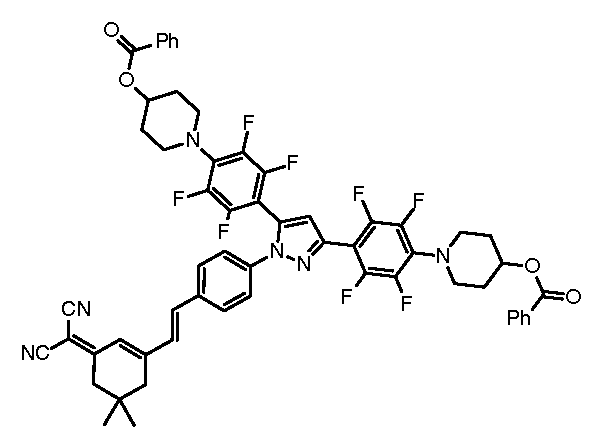
\includegraphics{sections/results/img/pyrazole1.eps}
    \caption{Структура полученного пиразола~\cmpd{pyrazole}}
    \label{fig:pyrazole1}
\end{figure}

Также мы наблюдали окисление пиразолина~\cmpd{decafluoropyrazoline_piperidine_DCIF.benzoyl} в пиразол даже при кратковременной выдержке в темноте в хлорированных растворителях~(\ce{CH2Cl2} и \ce{CDCl3}).
При этом для предшественника соединения~\cmpd{decafluoropyrazoline_piperidine_DCIF.benzoyl}~--- альдегида~\cmpd{decafluoropyrazoline_substituted.piperidine} окисления не наблюдалось даже при длительной выдержке в хлороформе на свету.
Это может быть связано с предполагаемым механизмом окисления~(\ref{sch:light_oxidation} на стр.\,\pageref{sch:light_oxidation}); введение в молекулу акцептора упрощает образование цвиттерионной структуры, играющей ключевую роль в процессе окисления.
В дальнейшем при получении производных соединения~\cmpd{decafluoropyrazoline_substituted.piperidine} мы старались избегать хлорсодержащих растворителей и длительного пребывания этих соединений на свету.

\subsection{Синтез красителей}

% По оптимизированной методике~(\ref{sch:cond_ac}) мы синтезировали производные соединений и~ с разделительными блоками~(\ref{fig:dendroids})~--- эфиры~\cmpd{decafluoropyrazoline_piperidine_DCIF.{benzoyl, TAFS, TATBS}} и~\cmpd{pentafluoropyrazoline_piperidine_DCIF.{benzoyl, TAFS, TATBS, IDATBS}}.

Найденные оптимальные условия ацилирования были применены для введения разветвленных заместителей\footnote{Реагенты в виде кислот и хлорангидридов предоставлены сотрудниками НИОХ Максимовым~А.М., Бережной~В.Н. и Рязановым~Н.Д.} в структуру красителей.
Кроме синтезированного в работе красителя~\cmpd{decafluoropyrazoline_DCIF.piperidine}, был использован полученный ранее в лаборатории краситель~\cmpd{pentafluoropyrazoline_DCIF.piperidine}\footnote{Соединение предоставлено сотрудником НИОХ Каргаполовой~И.Ю.}, содержащий одно 4-гидроксипиперидинозамещенное тетрафторфенильное кольцо.

\begin{scheme}[h!]
    \centering
    \begin{overpic}{sections/results/img/cond_ac.eps}
        \put(21.5, 58.1){\cmpd{decafluoropyrazoline_DCIF.piperidine}}
        \put(47, 58.1){\cmpd{decafluoropyrazoline_piperidine_DCIF.{benzoyl, TAFS, TATBS}}}
        \put(23, 8){\cmpd{pentafluoropyrazoline_DCIF.piperidine}}
        \put(76, 6){\cmpd{pentafluoropyrazoline_piperidine_DCIF.{benzoyl, TAFS, TATBS, IDATBS}}}
    \end{overpic}
    \caption{}
    \label{sch:cond_ac}
\end{scheme}

\begin{table}[h!]
    \centering
    \caption{Условия ацилирования соединений~\cmpd{decafluoropyrazoline_substituted.piperidine},~\cmpd{decafluoropyrazoline_DCIF.piperidine} и~\cmpd{pentafluoropyrazoline_DCIF.piperidine} и выходы продуктов}
    \label{tab:acylation_bis}
    \begin{small}
        \begin{threeparttable}
            \begin{tabular}{ccccccc}
                \toprule{}
                Субстрат                                           & Реагент        & \thead{Экв.                                                                                                               \\ реагента} & \thead{Условия\\ реакции}                 & \thead{Время\\ реакции, ч} & Продукт                                              & Выход, \% \\
                \midrule{}
                \cmpd{decafluoropyrazoline_substituted.piperidine} & \ce{PhCOCl}    & 6           & \ce{PhH}, \ce{Et3N}             & 24           & \cmpd{decafluoropyrazoline_piperidine_benzoyl}       & 74  \\
                \cmpd{decafluoropyrazoline_substituted.piperidine} & \ce{PhCOCl}    & 3           & \ce{PhH}, \ce{Et3N}, \ac{dmap}  & 6            & \cmpd{decafluoropyrazoline_piperidine_benzoyl}       & 74  \\
                \cmpd{decafluoropyrazoline_DCIF.piperidine}        & \ce{PhCOCl}    & 3           & \ce{PhH}, \ce{Et3N}, \ac{dmap}  & 1            & \cmpd{decafluoropyrazoline_piperidine_DCIF.benzoyl}  & 25  \\
                \cmpd{decafluoropyrazoline_DCIF.piperidine}        & \ce{TAFS-Cl}   & 3           & \ce{PhH}, \ce{Et3N}, \ac{dmap}  & 2            & \cmpd{decafluoropyrazoline_piperidine_DCIF.TAFS}     & 30  \\
                \cmpd{decafluoropyrazoline_DCIF.piperidine}        & \ce{TATBS-Cl}  & 3           & \ce{PhH}, \ce{Et3N}, \ac{dmap}  & 6            & \cmpd{decafluoropyrazoline_piperidine_DCIF.TATBS}    & 55  \\
                \cmpd{pentafluoropyrazoline_DCIF.piperidine}       & \ce{PhCOCl}    & 1.5         & \ce{PhH}, \ce{Et3N}, \ac{dmap}  & 4            & \cmpd{pentafluoropyrazoline_piperidine_DCIF.benzoyl} & 92  \\
                \cmpd{pentafluoropyrazoline_DCIF.piperidine}       & \ce{TAFS-Cl}   & 1.5         & \ce{PhH}, \ce{Et3N}, \ac{dmap}  & 2.5          & \cmpd{pentafluoropyrazoline_piperidine_DCIF.TAFS}    & 97  \\
                \cmpd{pentafluoropyrazoline_DCIF.piperidine}       & \ce{TATBS-Cl}  & 1.5         & \ce{PhH}, \ce{Et3N}, \ac{dmap}  & 3            & \cmpd{pentafluoropyrazoline_piperidine_DCIF.TATBS}   & 59  \\
                \cmpd{pentafluoropyrazoline_DCIF.piperidine}       & \ce{TATBS-OH}  & 1           & ТГФ, \ac{diad}, \ce{PPh3}       & 3            & \cmpd{pentafluoropyrazoline_piperidine_DCIF.TATBS}   & 70  \\
                \cmpd{pentafluoropyrazoline_DCIF.piperidine}       & \ce{TATBS-OH}  & 1           & \ce{PhH}, \ac{dcc}, \ac{dmap}   & 3            & \cmpd{pentafluoropyrazoline_piperidine_DCIF.TATBS}   & 22  \\
                \cmpd{pentafluoropyrazoline_DCIF.piperidine}       & \ce{IDATBS-Cl} & 1.5         & \ce{PhH}, \ce{Et3N}, \ac{dmap}  & 12           & \cmpd{pentafluoropyrazoline_piperidine_DCIF.IDATBS}  & 7.5 \\
                \cmpd{pentafluoropyrazoline_DCIF.piperidine}       & \ce{IDATBS-Cl} & 1.5         & \ce{MeCN}, \ce{Et3N}, \ac{dmap} & 36           & \cmpd{pentafluoropyrazoline_piperidine_DCIF.IDATBS}  & 7.5 \\
                \cmpd{pentafluoropyrazoline_DCIF.piperidine}       & \ce{IDATBS-Cl} & 1.5         & \ce{PhMe}, \ce{Et3N}, \ac{dmap} & 0.5\tnote{1} & \cmpd{pentafluoropyrazoline_piperidine_DCIF.IDATBS}  & 2.5 \\
                \bottomrule{}
            \end{tabular}
            \begin{tablenotes}
                \item[1]Реакцию проводили в микроволновом реакторе при температуре \SI{150}{\celsius}
            \end{tablenotes}
        \end{threeparttable}
    \end{small}
\end{table}

В целом, реакция ацилирования идет достаточно быстро и с хорошим выходом~(\ref{tab:acylation_bis}), однако при получении соединения~\cmpd{pentafluoropyrazoline_piperidine_DCIF.IDATBS} реакция не идет до конца, основной выделенный из реакционной смеси продукт~--- исходный краситель~\cmpd{pentafluoropyrazoline_DCIF.piperidine}.
Это может быть связано с тем, что хлорангидрид~\ce{IDATBS-Cl} является стерически затрудненным, а следовательно, затруднен подход OH-группы к карбонильной группе.
Для получения соединения~\cmpd{pentafluoropyrazoline_piperidine_DCIF.IDATBS} мы использовали несколько вариаций общей методики: увеличение времени реакции, замена растворителя с бензола на ацетонитрил, проведение реакции при повышенной температуре с нагревом микроволновым излучением, однако это не привело к повышению выхода.

% Также на то, что реакция проходит не до конца, указывает получение при очистке реакционной смеси желтой фракции, содержащей по данным ЯМР- и ИК-спектроскопии смесь исходного хлорангидрида и соответствующий кислоты.

В качестве альтернативных способов получения целевых эфиров мы также исследовали реакцию Мицунобу и реакцию Штеглиха~(взаимодействие спирта с кислотой в присутствим \ac{dcc} и \ac{dmap}). Реакция Штеглиха дает выход даже ниже, чем простое ацилирование хлорангидридом \todo{надо как-то объяснить}.

Реакция Мицунобу позволяет получать эфиры из спиртов и карбоновых кислот в присутствим диизопропилазодикарбоксилата~(\ac{diad}) и трифенилфосфина.
Применение этой реакции для получения соединения~\cmpd{pentafluoropyrazoline_piperidine_DCIF.TATBS} позволило еще больше снизить требуемое количество ацилирующего реагента~(в реакции Мицунобу он берется эквимолярно) и получить целевое соединение с большим выходом~(\ref{tab:acylation_bis}), чем при ацилировании с помощью хлорангидрида, а также позволяет использовать для ацилирования более доступную кислоту вместо ее хлорангидрида~(\ref{tab:acylation_bis}).

\begin{scheme}
    \centering
    \begin{overpic}{sections/results/img/mitsunobu.eps}
        \put(10, 42.5){\cmpd{pentafluoropyrazoline_DCIF.piperidine}}
        \put(91, 42.5){\cmpd{pentafluoropyrazoline_piperidine_DCIF.TATBS}}
    \end{overpic}
    \caption{}
    \label{sch:mitsunobu}
\end{scheme}

В спектрах ЯМР~\ce{^1H} соединений~\cmpd{pentafluoropyrazoline_piperidine_DCIF.{TAFS, TATBS, IDATBS}} наблюдается сигнал около \SI{4.2}{\ppm}, соответствующий \ce{S-CH2} фрагменту разделительного блока и сигналы около \SI{2.5}{\ppm}, принадлежащие метильным группам в ароматическом кольце.
В спектрах соединений~\cmpd{pentafluoropyrazoline_piperidine_DCIF.{TATBS, IDATBS}} присутствует сигнал \emph{трет}-бутильной группы при \SI{1.2}{\ppm}.
% Ароматические протоны основного \todo{подобрать слово} кольца в соединениях \cmpd{pentafluoropyrazoline_piperidine_DCIF.{TAFS, TATBS}} проявляются в виде синглета при 7.7--\SI{7.8}{\ppm}.
В спектрах соединений~\cmpd{decafluoropyrazoline_piperidine_DCIF.{benzoyl, TAFS, TATBS}} описанные сигналы выглядят как дублеты из-за неэквивалентности двух заместителей.
Спектры ЯМР \ce{^19F} соединений~\cmpd{decafluoropyrazoline_piperidine_DCIF.{TAFS}} и~\cmpd{pentafluoropyrazoline_piperidine_DCIF.{TAFS}} соответствуют структуре красителей с TAFS-фрагментом.

Синтезированные красители имеют длинноволновый максимум поглощения при длине волны 490--\SI{500}{\nano\metre} в ацетоне, который не зависит от структуры введенного разделительного блока, поскольку тот не включен в цепь сопряжения~(\ref{fig:1OH-UV}).

\begin{figure}[h!]
    \centering
    \subfigure[Cоединения~\cmpd{decafluoropyrazoline_piperidine_DCIF.{benzoyl, TAFS}}]
    {
    \begin{overpic}[width = 0.45\textwidth]{sections/results/img/2OH - Copy.pdf}
        \put(92,82.5){\scriptsize\cmpd{decafluoropyrazoline_piperidine_DCIF.benzoyl}}
        \put(92,78.0){\scriptsize\cmpd{decafluoropyrazoline_piperidine_DCIF.TAFS}}
    \end{overpic}
    }
    \subfigure[Соединения~\cmpd{pentafluoropyrazoline_piperidine_DCIF.{benzoyl, TAFS, TATBS, IDATBS}}]
    {
    \begin{overpic}[width = 0.45\textwidth]{sections/results/img/1OH - Copy.eps}
        \put(92,83){\scriptsize\cmpd{pentafluoropyrazoline_piperidine_DCIF.IDATBS}}
        \put(92,78.5){\scriptsize\cmpd{pentafluoropyrazoline_piperidine_DCIF.TATBS}}
        \put(92,74){\scriptsize\cmpd{pentafluoropyrazoline_piperidine_DCIF.TAFS}}
        \put(92,70){\scriptsize\cmpd{pentafluoropyrazoline_piperidine_DCIF.benzoyl}}
    \end{overpic}
    }
    \caption{Нормированные электронные спектры поглощения полученных красителей}
    \label{fig:1OH-UV}
\end{figure}

Полученные красители обладают флуоресценцией с максимумом возбуждения около \SI{490}{\nano\metre} и стоксовым сдвигом около \SI{210}{\nano\metre}

\begin{figure}[h!]
    \centering
    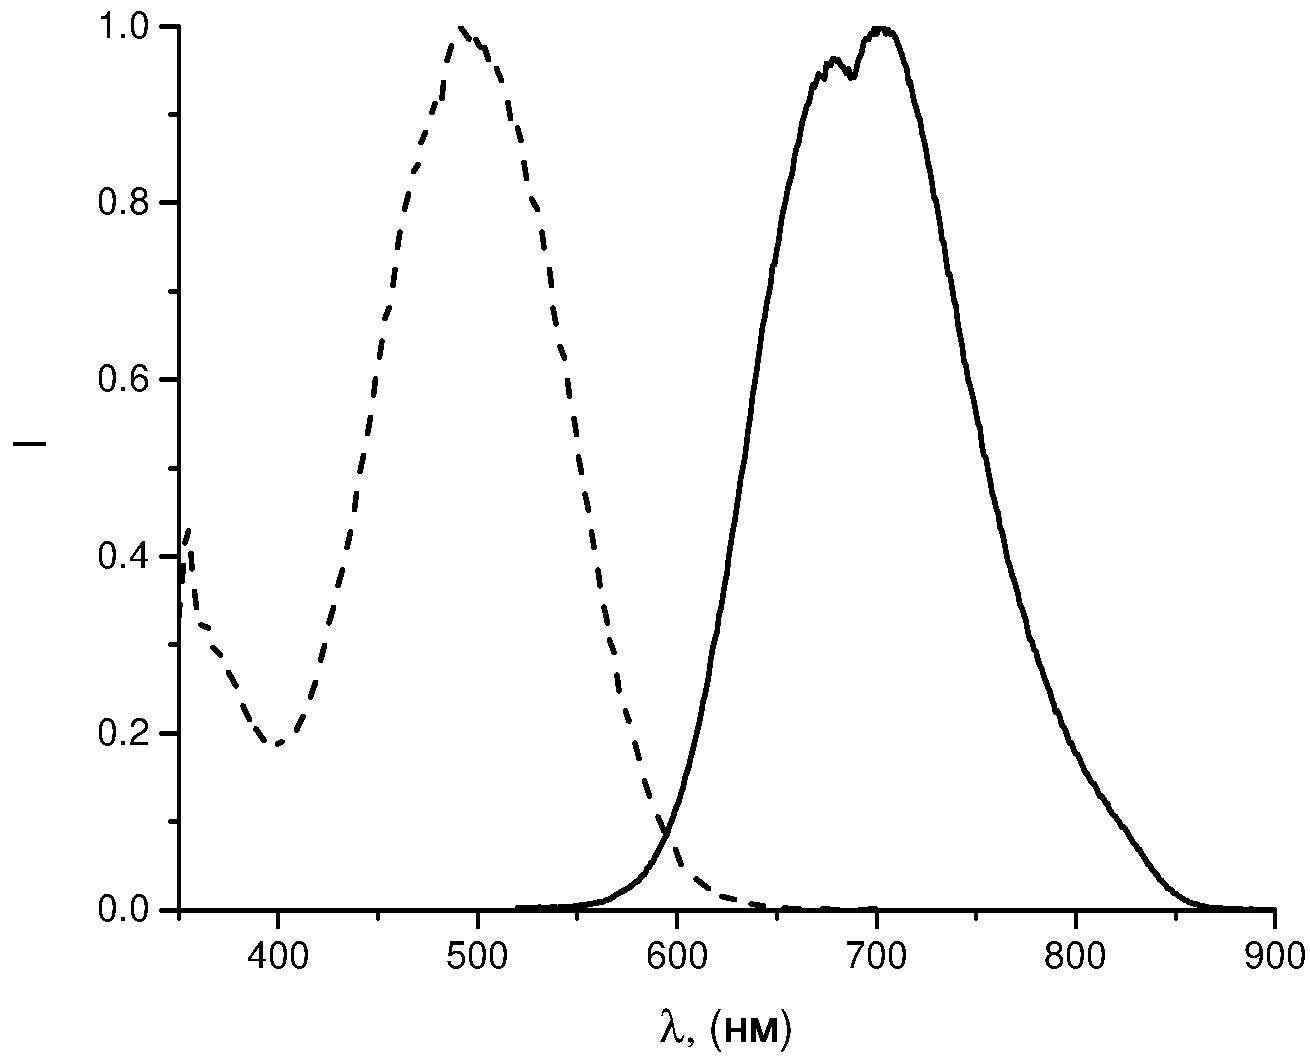
\includegraphics[width = 0.5\textwidth]{sections/results/img/Graph3 - Copy.pdf}
    \caption{Спектры флуоресценции~(сплошная линия) и возбуждения флуоресценции~(пунктирная линия) соединения~\cmpd{decafluoropyrazoline_piperidine_DCIF.TAFS}}
\end{figure} \todo{надо бы еще в разных растворителях}

\begin{center}
    \LARGE
    \textbf{***}
\end{center}

Таким образом, в работе полностью выполнена поставленная цель по синтезу новых донорно-акцепторных красителей, содержащих в качестве донорных блоков производные полифтортриарилпиразолинов с разветвленными фрагментами на основе п-толуиловой и β-изодуриловой кислот.
В ходе исследования выявлены рациональные последовательности стадий синтеза и найдены оптимальные условия модификации красителей разветвленными группами.